% !TeX root = thesis.tex

\chapter{Results} \label{chap:results}

This chapter presents the experimental results obtained for the three model families developed in this
dissertation, the traditional ML baselines, the single-task LSTM models and the two multi-task LSTM
architectures, across the window sizes tested and the three tasks addressed: AD, FD, and PdM.

Results are organized by task rather than by model family, so that the traditional baselines, the
single-task models, and the two multi-task architectures can be compared directly with one another within
each task. Section~\ref{sec:results_ad} presents the AD results,
Section~\ref{sec:results_fd} the FD results, and Section~\ref{sec:results_pdm} the PdM results. 
Section~\ref{sec:results_summary} closes the chapter with an objective summary of the
patterns observed across all three tasks, without yet interpreting their causes, which is left to the
Discussion Chapter.

The DL models were evaluated across all eleven window sizes, from 1 to 1{,}024 observations. The 
traditional baselines were evaluated up to a window size of 128 for AD and FD, and up to 64 for PdM, 
within the computational budget available for this dissertation: a single grouped cross-validated grid 
search for the Random Forest regressor already required over eighty minutes. Entries beyond these limits 
are therefore reported as unavailable rather than as missing results. In every table, the best value obtained
by each model across the window sizes tested is set in bold.

\section{Anomaly Detection Results} \label{sec:results_ad}

Table~\ref{tab:results_ad_f1} presents the F1-score obtained for AD by each model and
window size. Figure~\ref{fig:results_ad} shows the same results graphically.

\begin{table}[htbp]
\centering
\caption{Anomaly detection F1-score by model and window size.}
\label{tab:results_ad_f1}
\small
% Auto-generated by results.ipynb -- do not edit by hand
\begin{tabular}{lrrrrr}
\hline
\textbf{Window size} & \textbf{Random Forest} & \textbf{XGBoost} & \textbf{STL} & \textbf{MTL (joint)} & \textbf{MTL (cascaded)} \\
\hline
1 & 0.239 & 0.248 & 0.836 & 0.798 & 0.806 \\
2 & 0.268 & 0.273 & 0.814 & 0.810 & 0.802 \\
4 & 0.289 & 0.313 & 0.805 & 0.805 & 0.812 \\
8 & 0.315 & 0.352 & 0.814 & 0.857 & 0.822 \\
16 & 0.419 & 0.420 & 0.781 & 0.822 & 0.832 \\
32 & \textbf{0.441} & \textbf{0.460} & 0.865 & 0.868 & 0.850 \\
64 & 0.396 & 0.347 & \textbf{0.900} & 0.826 & 0.872 \\
128 & 0.353 & 0.328 & 0.857 & \textbf{0.885} & \textbf{0.889} \\
256 & -- & -- & 0.897 & 0.881 & 0.871 \\
512 & -- & -- & 0.899 & 0.761 & 0.885 \\
1,024 & -- & -- & 0.823 & 0.838 & 0.854 \\
\hline
\end{tabular}

\end{table}

\begin{figure}[htbp]
    \centering
    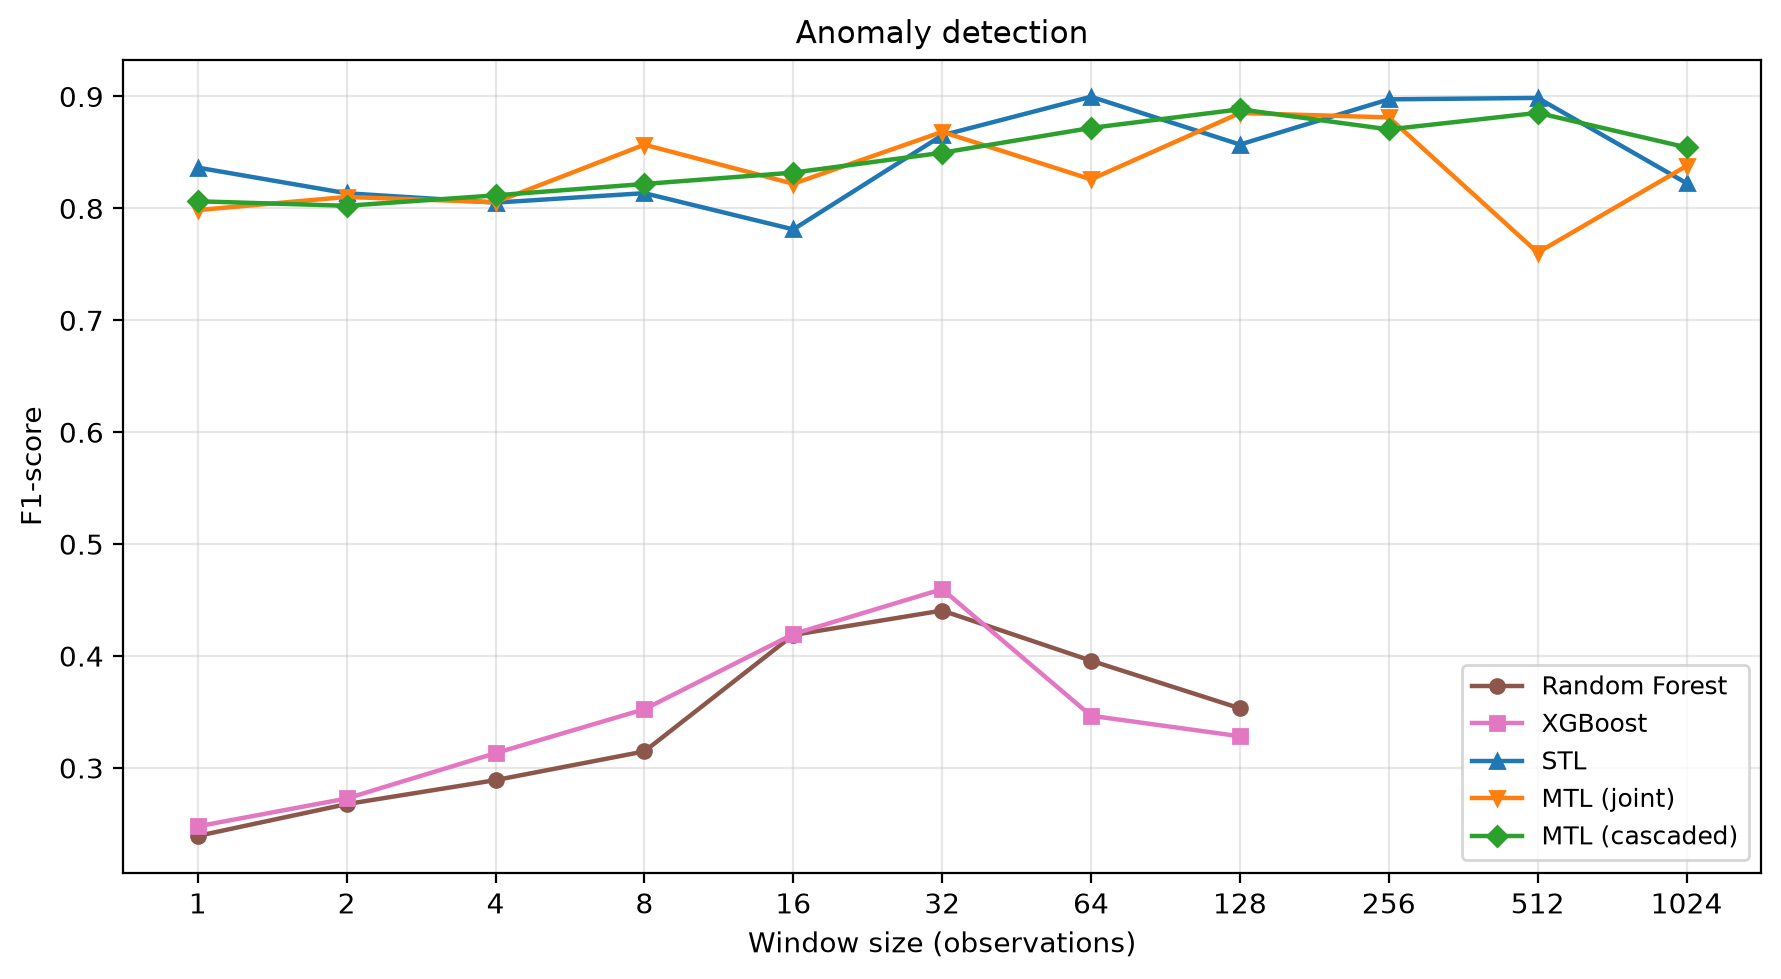
\includegraphics[width=0.85\textwidth]{imgs/results_ad_f1.png}
    \caption{Anomaly detection F1-score against window size, for all five models.}
    \label{fig:results_ad}
\end{figure}

The three DL models separate clearly from the two traditional baselines at every window size
tested. The lowest F1-score obtained by any DL model, 0.761 for the joint multi-task
architecture at a window size of 512, remains above the highest F1-score obtained by either baseline,
0.460 for XGBoost at a window size of 32. Across the window sizes where all five models are available, the
DL models score roughly twice as high as the baselines.

The single-task model reaches the highest F1-score observed across all models and window sizes, 0.900 at a
window size of 64, followed closely by the cascaded multi-task architecture at 0.889 and the joint
architecture at 0.885, both at a window size of 128. The difference between these three best
configurations is 0.015.

The two families respond differently to the amount of temporal context available. The baselines improve
from a window size of 1 up to 32, where both peak, and then decline: Random Forest falls from 0.441 to
0.353 and XGBoost from 0.460 to 0.328 between window sizes 32 and 128. The DL models remain
comparatively flat, varying between 0.761 and 0.900 across the entire range. Notably, all three DL models already exceed 0.79 at a window size of 1, where no
temporal context is available at all.

Table~\ref{tab:results_ad_roc} reports the corresponding area under the ROC curve, which is independent of
the decision threshold applied.

\begin{table}[htbp]
\centering
\caption{Anomaly detection ROC-AUC by model and window size.}
\label{tab:results_ad_roc}
\small
% Auto-generated by results.ipynb -- do not edit by hand
\begin{tabular}{lrrrrr}
\hline
\textbf{Window size} & \textbf{Random Forest} & \textbf{XGBoost} & \textbf{STL} & \textbf{MTL (joint)} & \textbf{MTL (cascaded)} \\
\hline
1 & 0.797 & 0.744 & 0.978 & 0.975 & 0.975 \\
2 & 0.824 & 0.803 & 0.981 & \textbf{0.982} & 0.971 \\
4 & 0.836 & 0.820 & 0.955 & 0.978 & 0.966 \\
8 & 0.810 & 0.856 & \textbf{0.985} & 0.969 & 0.979 \\
16 & 0.878 & 0.873 & 0.928 & 0.972 & 0.974 \\
32 & 0.885 & \textbf{0.909} & 0.958 & 0.979 & 0.971 \\
64 & 0.877 & 0.888 & 0.983 & 0.974 & 0.977 \\
128 & \textbf{0.889} & 0.878 & 0.984 & 0.972 & \textbf{0.983} \\
256 & -- & -- & 0.978 & 0.972 & 0.979 \\
512 & -- & -- & 0.974 & 0.943 & 0.973 \\
1,024 & -- & -- & 0.939 & 0.958 & 0.976 \\
\hline
\end{tabular}

\end{table}

The same separation is visible in the ROC-AUC, though compressed by the upper bound of the metric. The
deep learning models range from 0.928 to 0.985 across all window sizes, while the baselines range from
0.744 to 0.909. The highest value is 0.985, obtained by the single-task model at a window size of 8, and
the highest value obtained by a baseline is 0.909, by XGBoost at a window size of 32.

\section{Fault Detection Results} \label{sec:results_fd}

Table~\ref{tab:results_fd_f1} presents the mean F1-score across the four fault types and Figure~\ref{fig:results_fd} shows the same results
graphically.

\begin{table}[htbp]
\centering
\caption{Fault detection mean F1-score by model and window size.}
\label{tab:results_fd_f1}
\small
% Auto-generated by results.ipynb -- do not edit by hand
\begin{tabular}{lrrrrr}
\hline
\textbf{Window size} & \textbf{Random Forest} & \textbf{XGBoost} & \textbf{STL} & \textbf{MTL (joint)} & \textbf{MTL (cascaded)} \\
\hline
1 & 0.248 & 0.226 & 0.545 & 0.584 & 0.544 \\
2 & 0.256 & 0.238 & 0.511 & 0.587 & 0.563 \\
4 & 0.274 & 0.320 & 0.516 & 0.492 & 0.521 \\
8 & 0.358 & 0.354 & 0.623 & 0.605 & 0.562 \\
16 & 0.439 & 0.422 & \textbf{0.701} & 0.602 & 0.553 \\
32 & \textbf{0.483} & 0.471 & 0.572 & 0.579 & 0.613 \\
64 & 0.475 & \textbf{0.504} & 0.553 & 0.626 & \textbf{0.720} \\
128 & 0.465 & 0.323 & 0.578 & 0.604 & 0.569 \\
256 & -- & -- & 0.560 & \textbf{0.640} & 0.670 \\
512 & -- & -- & 0.687 & 0.621 & 0.563 \\
1,024 & -- & -- & 0.578 & 0.584 & 0.598 \\
\hline
\end{tabular}

\end{table}

\begin{figure}[htbp]
    \centering
    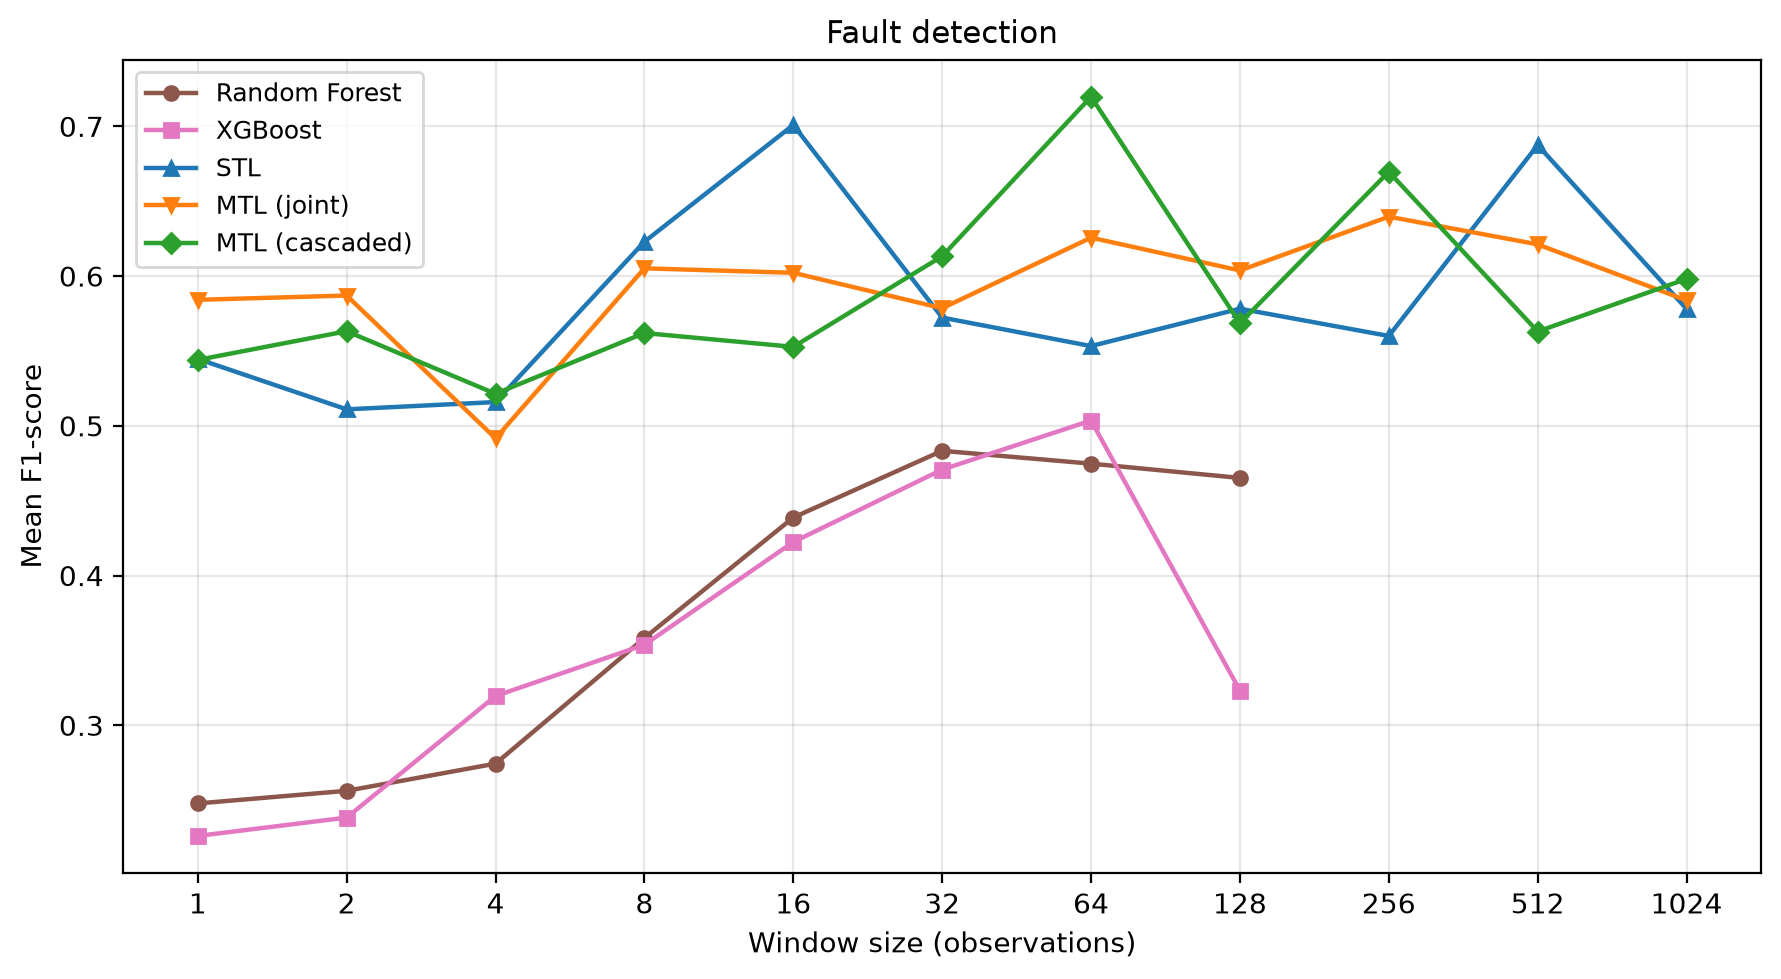
\includegraphics[width=0.85\textwidth]{imgs/results_fd_f1.png}
    \caption{Fault detection mean F1-score against window size, for all five models.}
    \label{fig:results_fd}
\end{figure}

The cascaded multi-task architecture reaches the highest mean F1-score observed across all models and
window sizes, 0.720 at a window size of 64. The single-task model follows at 0.701, obtained at a window
size of 16, and the joint architecture at 0.640, at a window size of 256. The best values obtained by the
baselines are lower, 0.504 for XGBoost at a window size of 64 and 0.483 for Random Forest at 32.

The margin between the DL models and the baselines is narrower here than for anomaly detection,
and is not uniform across window sizes. At window sizes of 4 and below, XGBoost scores between 0.226 and
0.320 while the DL models score between 0.492 and 0.587. At a window size of 32, however,
Random Forest reaches 0.483 against 0.572 for the single-task model, and the cascaded architecture drops
to 0.613, its second lowest value.

The DL models exhibit considerable variation across window sizes, with no clear trend. This contrasts with the baseline models, 
which show a consistent trend before their performance drops after a window size of 64.

Table~\ref{tab:results_fd_perfault} breaks the results down by individual fault type, taking each model at
its own best-performing window size identified above, and Figure~\ref{fig:results_fd_perfault} presents
the same breakdown graphically.

\begin{table}[htbp]
\centering
\caption{Fault detection F1-score per fault type, with each model taken at its best window size.}
\label{tab:results_fd_perfault}
\scriptsize
% Auto-generated by results.ipynb -- do not edit by hand
\begin{tabular}{lrrrrr}
\hline
\textbf{Fault type} & \textbf{Random Forest (ws=32)} & \textbf{XGBoost (ws=64)} & \textbf{STL (ws=16)} & \textbf{MTL (joint) (ws=256)} & \textbf{MTL (cascaded) (ws=64)} \\
\hline
Clogged filters & 0.079 & 0.142 & 0.769 & 0.792 & 0.841 \\
Cooling fault & 0.723 & 0.758 & 0.828 & 0.810 & 0.815 \\
Valve fault & 0.634 & 0.630 & 0.688 & 0.660 & 0.855 \\
Bearing fault & 0.498 & 0.484 & 0.518 & 0.297 & 0.368 \\
\hline
\end{tabular}

\end{table}

\begin{figure}[htbp]
    \centering
    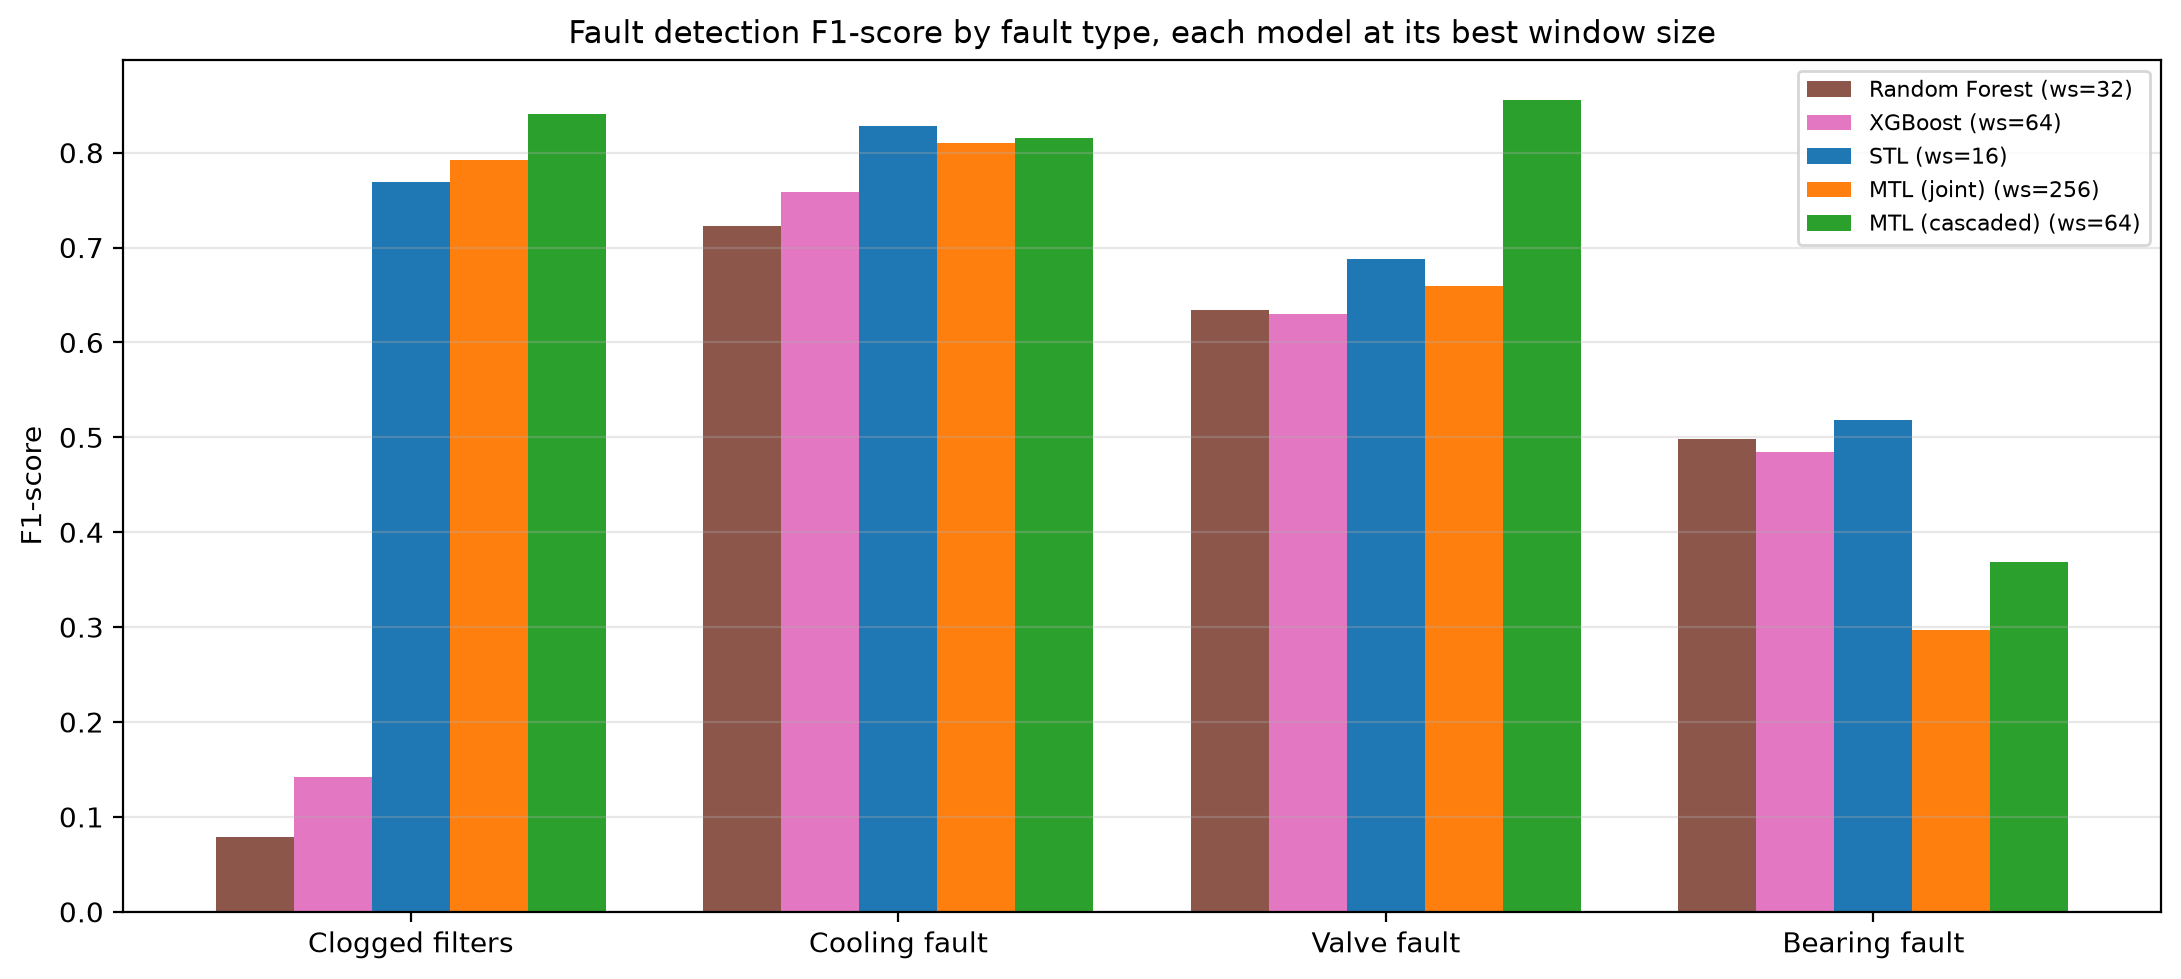
\includegraphics[width=0.9\textwidth]{imgs/results_fd_perfault.png}
    \caption{Fault detection F1-score by fault type, with each model taken at its best window size.}
    \label{fig:results_fd_perfault}
\end{figure}

The breakdown shows that the aggregate mean F1-score conceals two opposite patterns. The clogged filters
fault separates the two families most sharply: the baselines obtain 0.079 for Random Forest and 0.142 for
XGBoost, the lowest values recorded for any fault type and any model, while the three DL models
obtain between 0.769 and 0.841 on the same fault. The bearing fault reverses this ordering: the baselines
obtain 0.498 and 0.484, above the 0.297 of the joint architecture and the 0.368 of the cascaded
architecture, with only the single-task model higher at 0.518.

The cooling fault is the most consistently detected across all five models, with F1-scores between 0.723
and 0.828 and a spread of only 0.105 between the best and worst model. The valve fault shows the widest
spread, from 0.630 for XGBoost to 0.855 for the cascaded architecture.

Considering the balance across fault types rather than the average, the single-task model at a window size
of 16 shows the narrowest range, from 0.518 to 0.828. The two baselines show the widest, both spanning
more than 0.6 between their best and worst fault type, driven entirely by their result on the clogged
filters fault.

\section{Predictive Maintenance Results} \label{sec:results_pdm}

Table~\ref{tab:results_pdm_mae} presents the mean absolute error obtained for predictive maintenance and
Table~\ref{tab:results_pdm_r2} the corresponding coefficient of determination. Figure~\ref{fig:results_pdm} shows both metrics against window size.

\begin{table}[htbp]
\centering
\caption{Predictive maintenance MAE by model and window size.}
\label{tab:results_pdm_mae}
\small
% Auto-generated by results.ipynb -- do not edit by hand
\begin{tabular}{lrrrrr}
\hline
\textbf{Window size} & \textbf{Random Forest} & \textbf{XGBoost} & \textbf{STL} & \textbf{MTL (joint)} & \textbf{MTL (cascaded)} \\
\hline
1 & 0.110 & 0.114 & 0.046 & 0.053 & 0.052 \\
2 & 0.106 & 0.136 & 0.049 & 0.050 & 0.053 \\
4 & 0.107 & 0.131 & 0.050 & 0.066 & 0.052 \\
8 & 0.095 & 0.127 & 0.049 & 0.051 & 0.051 \\
16 & \textbf{0.094} & 0.097 & 0.050 & 0.050 & 0.049 \\
32 & 0.114 & \textbf{0.096} & 0.046 & 0.053 & 0.047 \\
64 & 0.119 & 0.104 & 0.048 & 0.053 & \textbf{0.041} \\
128 & -- & -- & 0.039 & \textbf{0.048} & 0.044 \\
256 & -- & -- & \textbf{0.034} & 0.065 & 0.042 \\
512 & -- & -- & 0.049 & 0.065 & 0.043 \\
1,024 & -- & -- & 0.052 & 0.065 & 0.046 \\
\hline
\end{tabular}

\end{table}

\begin{table}[htbp]
\centering
\caption{Predictive maintenance $R^2$ by model and window size.}
\label{tab:results_pdm_r2}
\small
% Auto-generated by results.ipynb -- do not edit by hand
\begin{tabular}{lrrrrr}
\hline
\textbf{Window size} & \textbf{Random Forest} & \textbf{XGBoost} & \textbf{STL} & \textbf{MTL (joint)} & \textbf{MTL (cascaded)} \\
\hline
1 & -0.030 & 0.065 & 0.554 & 0.532 & 0.532 \\
2 & \textbf{0.018} & -0.274 & 0.483 & 0.563 & 0.489 \\
4 & -0.078 & -0.235 & 0.442 & 0.382 & 0.500 \\
8 & 0.018 & -0.179 & 0.495 & 0.545 & 0.590 \\
16 & -0.094 & \textbf{0.069} & 0.494 & \textbf{0.615} & 0.531 \\
32 & -0.420 & 0.004 & 0.477 & 0.511 & 0.571 \\
64 & -0.266 & -0.061 & 0.487 & 0.502 & 0.653 \\
128 & -- & -- & 0.578 & 0.594 & 0.630 \\
256 & -- & -- & \textbf{0.678} & 0.382 & \textbf{0.655} \\
512 & -- & -- & 0.494 & 0.356 & 0.651 \\
1,024 & -- & -- & 0.538 & 0.494 & 0.554 \\
\hline
\end{tabular}

\end{table}

\begin{figure}[htbp]
    \centering
    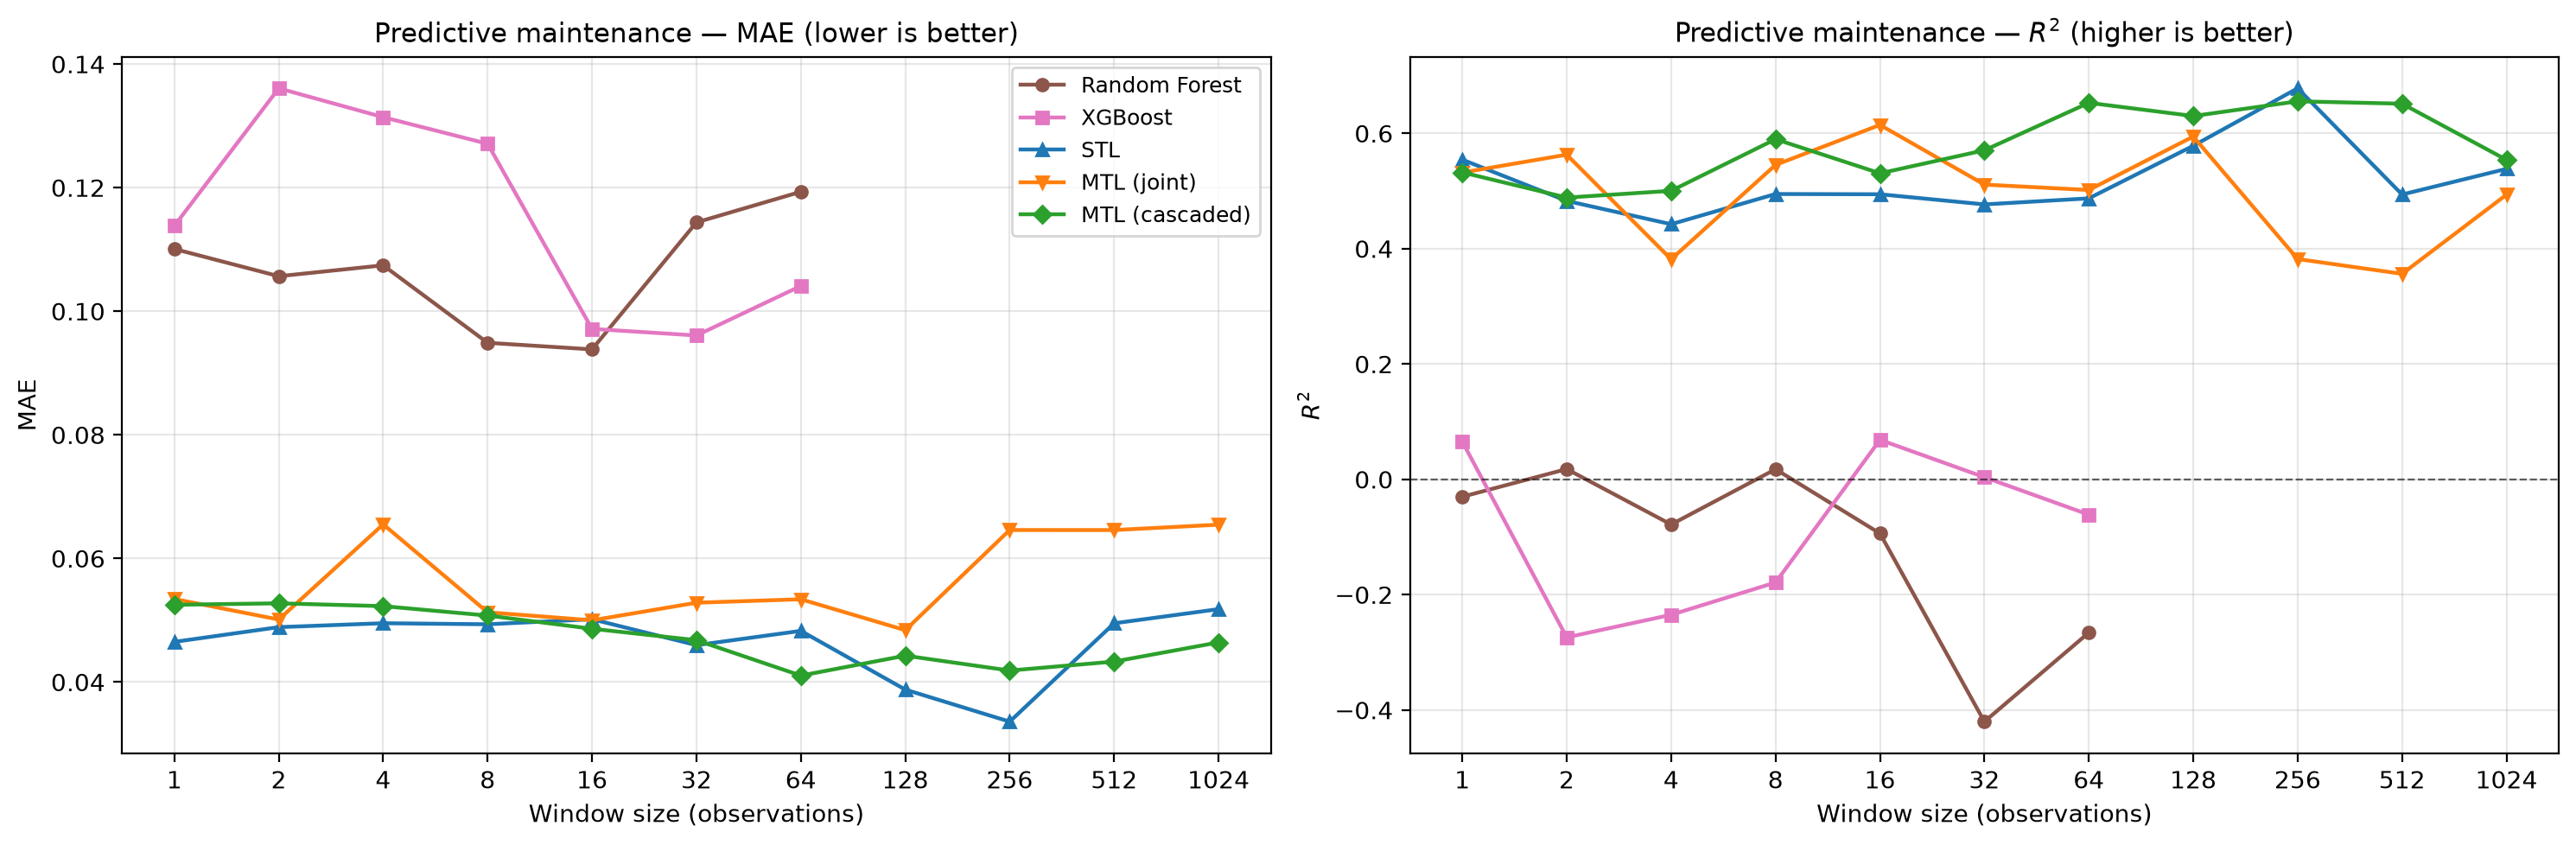
\includegraphics[width=0.98\textwidth]{imgs/results_pdm.png}
    \caption{Predictive maintenance MAE (left) and $R^2$ (right) against window size, for all five models.
    The dashed line on the right marks $R^2 = 0$, the value obtained by always predicting the mean
    severity of the training data.}
    \label{fig:results_pdm}
\end{figure}

This is the task where the two families separate most clearly. The three DL models obtain an
$R^2$ between 0.356 and 0.678 across every window size tested, while the two baselines obtain values
between $-0.420$ and $0.069$. The best baseline result, 0.069 for XGBoost at a window size of 16, is
therefore barely distinguishable from the performance of a model that always predicts the mean severity
observed in the training data, and both baselines produce a negative $R^2$ at the majority of window sizes
tested, meaning they perform worse than that constant predictor.

The MAE tells a consistent story. The DL models range from 0.034 to 0.066 across all window
sizes, while the baselines range from 0.094 to 0.136. The lowest MAE observed is 0.034, obtained by the
single-task model at a window size of 256, which is also the configuration producing the highest $R^2$,
0.678. The cascaded architecture follows with an MAE of 0.041 at a window size of 64 and an $R^2$ of 0.655
at 256.

Among the DL models, the joint architecture is the least stable on this task, with its $R^2$
falling from 0.615 at a window size of 16 to 0.356 at 512, and its MAE rising from 0.048 to 0.066 over the
same range. The cascaded architecture and the single-task model remain within a narrower band, between
0.442 and 0.678 in $R^2$ across all window sizes.

\section{Summary of Findings} \label{sec:results_summary}

This section summarizes, without yet interpreting, the main patterns observed across the three tasks and
five models compared in this chapter. Table~\ref{tab:results_best} collects the best configuration
obtained by each model on each task.

\begin{table}[htbp]
\centering
\caption{Best configuration obtained by each model on each task.}
\label{tab:results_best}
\small
% Auto-generated by results.ipynb -- do not edit by hand
\begin{tabular}{lllrr}
\hline
\textbf{Task} & \textbf{Metric} & \textbf{Model} & \textbf{Best window} & \textbf{Value} \\
\hline
Anomaly detection & F1-score & Random Forest & 32 & 0.441 \\
 &  & XGBoost & 32 & 0.460 \\
 &  & STL & 64 & 0.900 \\
 &  & MTL (joint) & 128 & 0.885 \\
 &  & MTL (cascaded) & 128 & 0.889 \\
\hline
Fault detection & Mean F1-score & Random Forest & 32 & 0.483 \\
 &  & XGBoost & 64 & 0.504 \\
 &  & STL & 16 & 0.701 \\
 &  & MTL (joint) & 256 & 0.640 \\
 &  & MTL (cascaded) & 64 & 0.720 \\
\hline
Predictive maint. & $R^2$ & Random Forest & 2 & 0.018 \\
 &  & XGBoost & 16 & 0.069 \\
 &  & STL & 256 & 0.678 \\
 &  & MTL (joint) & 16 & 0.615 \\
 &  & MTL (cascaded) & 256 & 0.655 \\
\hline
\end{tabular}

\end{table}

The three DL models outperformed the two traditional baselines on all three tasks.
No single model was best on all three tasks. The single-task models obtained the highest AD
F1-score (0.900 at a window size of 64) and the highest PdM $R^2$ (0.678 at 256), while
the cascaded multi-task architecture obtained the highest FD mean F1-score (0.720 at 64). In
each case the margin over the runner-up was small: 0.011 for AD, 0.019 for FD
and 0.023 for PdM.

Between the two multi-task architectures, the cascaded variant matched or exceeded the joint variant on
all three tasks, with the largest difference on FD (0.720 against 0.640) and the smallest on
AD (0.889 against 0.885).

The effect of window size differed by model family. The two baselines improved with increasing window size
up to 16 or 32 observations and then declined on both classification tasks, while the DL models
varied within a comparatively narrow band across the entire range and reached values above 0.79 for
AD even at a window size of 1, where no temporal context is available. No model obtained
its best result at the largest window size tested for any of the three tasks.

Across fault types, the clogged filters fault produced the widest disagreement between the two families,
with F1-scores of 0.079 and 0.142 for the baselines against 0.769 to 0.841 for the DL models.
The bearing fault was the hardest for the multi-task architectures, at 0.297 and 0.368, while both
baselines obtained higher values on that same fault.